\documentclass{labart}

\renewcommand{\abstractname}{概要}
\title{实验名称}  
\author{网络与系统安全综合实验}   
\date{实验截止: XXXX.xx.xx 星期X 23:59} 
\labtitle{lab1}

\begin{document}

\maketitle

% 本文件使用XeLaTeX编译生成,确保编译前已安装所需的Package

\begin{abstract}
这里是概要,可以写一些实验的背景或者简介
\begin{itemize}
\item[·] 这里是一个项目列表
\item[·] 第二项
\item[·] 第三项
\end{itemize}
\end{abstract}


\section{这是一个一级标题}
\subsection{这是一个二级标题}
可以说明此次实验的所有内容,比如:
本次课程一共有三个lab:
\begin{itemize}
\item[·] lab1:逆向实验
\item[·] lab2:shellcode\&栈溢出实验
\item[·] lab3:格式化字符串\&ROP实验
\end{itemize}

\subsection{提交内容(举例)}
每次lab实验需要提交实验报告(PDF/Word),实验报告需要完整反映题目解答过程和最后的答案。
如果编写了对应的解题脚本,连同脚本和实验报告一同压缩为.zip格式上交。

\begin{lstlisting}[numbers=none,frame=none]
命名格式:
压缩包:lab[1-3]-学号-姓名.zip                    e.g. lab1-17000000001-张三.zip
报告:  lab[1-3]-学号-姓名.[doc/pdf]              e.g. lab1-17000000001-张三.pdf
脚本:  lab[1-3]-[1-5]-学号-姓名.[c/py/...]       e.g. lab1-2-17000000001-张三.py
\end{lstlisting}


\section{这是另一个标题}
可以对实验使用的工具/内容进行详细说明。

如果要使用一个fig添加多张图片可以参考以下格式:
\begin{figure}[H] \centering    
\subfigure[IDA图标与待逆向文件] {
 \label{fig:a}     
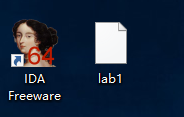
\includegraphics[width=0.2\columnwidth]{./lab/1.png}  
}     
\subfigure[IDA Quick start] { 
\label{fig:b}     
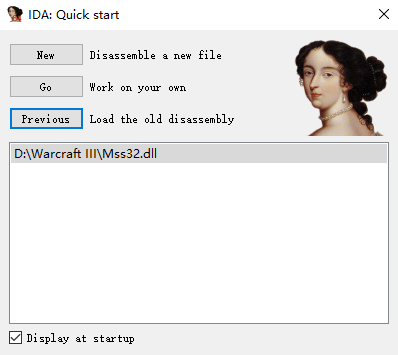
\includegraphics[width=0.2\columnwidth]{./lab/2.png}     
}    
\subfigure[文件选择] { 
\label{fig:b}     
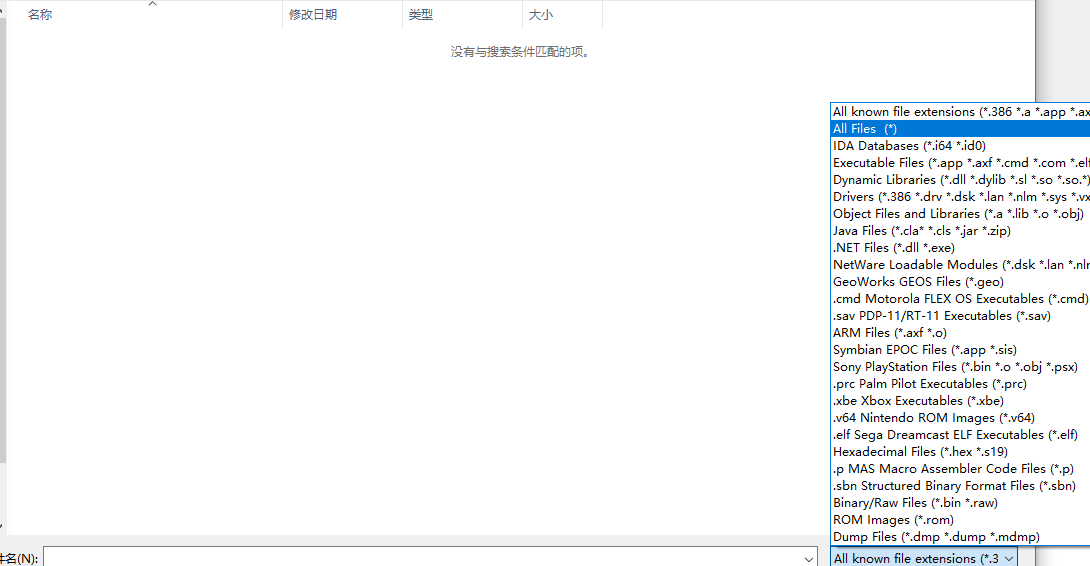
\includegraphics[width=0.2\columnwidth]{./lab/3.png}     
}   
\subfigure[选择指令集] { 
\label{fig:b}     
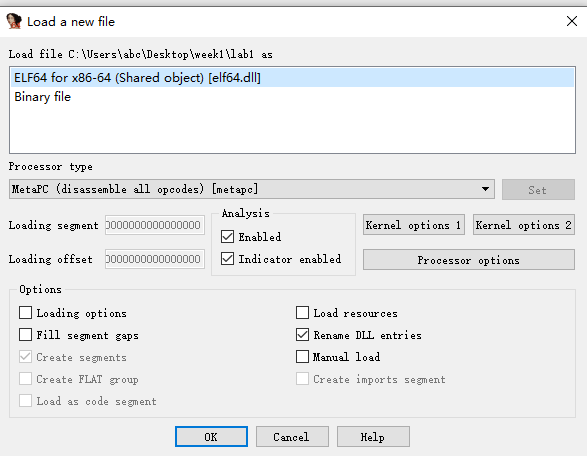
\includegraphics[width=0.2\columnwidth]{./lab/5.png}     
}   
\caption{ IDA打开文件过程 }     
\label{fig}     
\end{figure}

如果只添加一张图片,可以参考以下格式:

\begin{figure}[H]
\centering
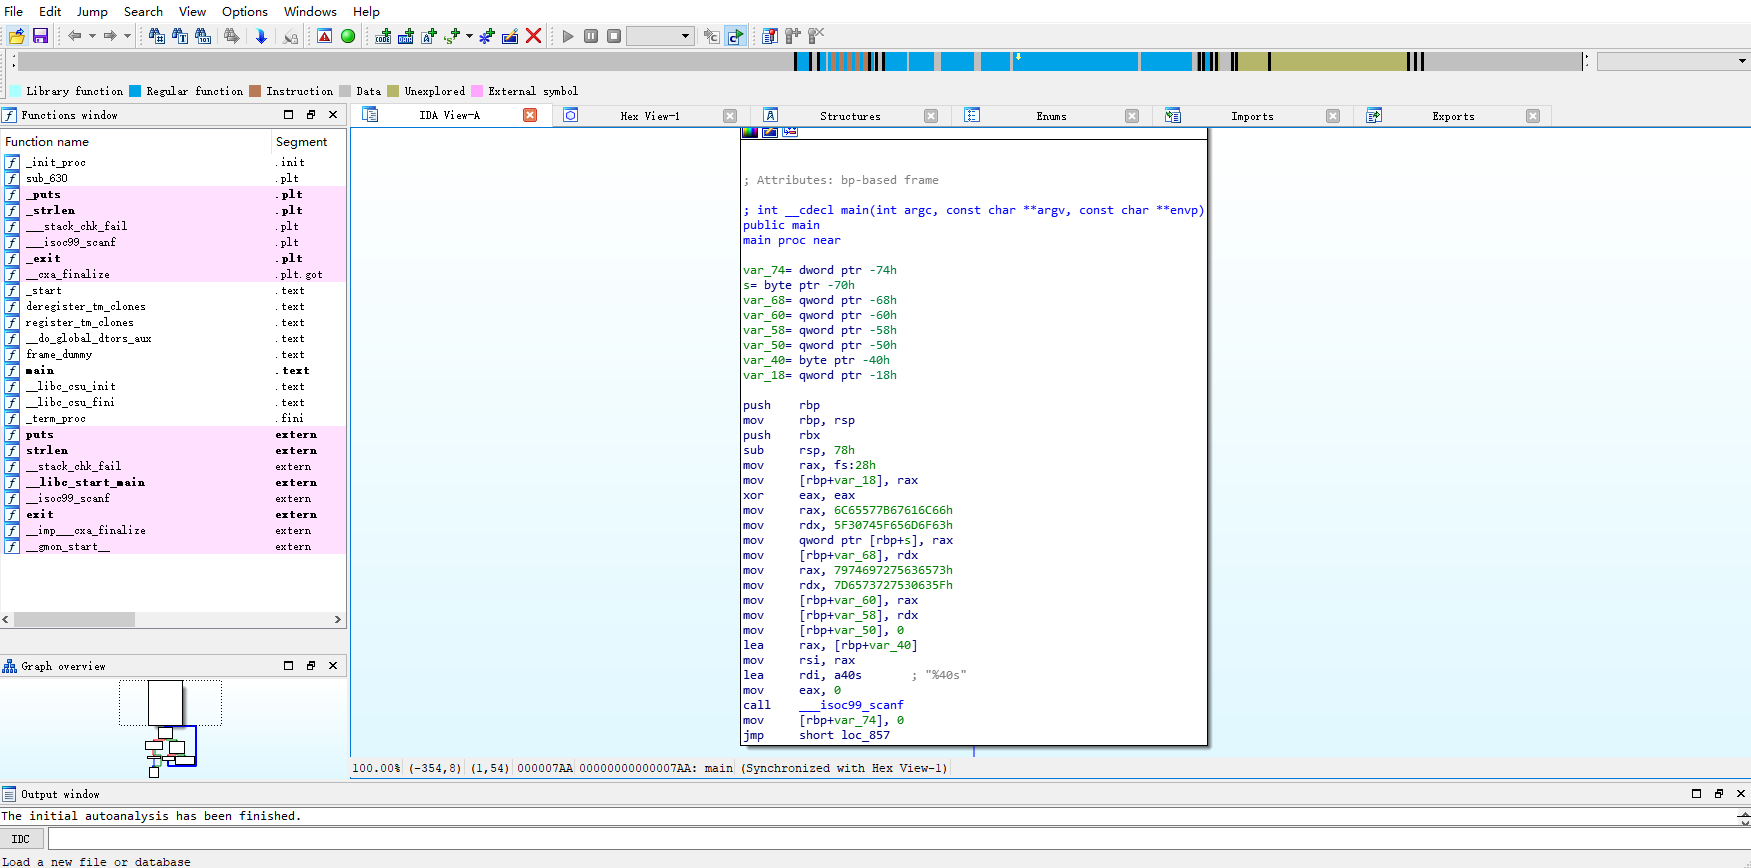
\includegraphics[scale=0.2]{./lab/6.png}
\caption{IDA界面}
\label{fig:label}
\end{figure}

如果要添加表格,可以参考以下格式:

\begin{table}[H]
\centering
\caption{gdb常用命令}
\begin{tabular}{|c|c|c|}
\hline  
命令&参数&含义\\
\hline  
run&&运行当前程序\\
\hline
break& 地址& 在参数所表示的地址处添加断点 \\
\hline 
continue&&从当前位置继续执行,直到遇到断点停止 \\
\hline
quit && 退出gdb \\
\hline
attach & 进程的pid & 使用gdb调试当前运行的程序 \\
\hline
n && set over,遇到函数不进入函数内部 \\
\hline
s && set into,遇到函数进入函数内部 \\
\hline
finish && step out,执行完并且退出当前函数 \\
\hline
info & registers & 显示所有寄存器 \\
\hline
info & b & 当前设置的断点 \\
\hline
del & 断点的序号 & 删除某个断点 \\
\hline 
x/nfu & 地址 & 以f格式打印从地址处开始的n个长度单元为u的内存值。\\
&&f:是输出格式。x:16进制,o:8进制。u:标明一个单元的长度。\\
&&b:一个byte,h:两个byte(halfword)\\
&&w:四个byte(word),g:八个byte(giant word)\\
\hline
vmmap(需要peda插件) && 打印调试程序的虚拟地址映射 \\
\hline
\end{tabular}
\end{table}

如果要插入代码可以参考以下格式:
\begin{lstlisting}[ language=Java]
    public static void main(String[] args) {
	    Scanner scanner = new Scanner(System.in);
	    int n = scanner.nextInt();
	    System.out.println(n);
    }
}
\end{lstlisting}



\end{document}